\documentclass[10pt, a4paper,english,spanish,hidelinks]{article}
\usepackage{amsmath}
\usepackage{amsfonts}
\usepackage{amssymb}
\usepackage{caratula}
\usepackage[spanish, activeacute]{babel}
\usepackage[usenames,dvipsnames]{color}
\usepackage[width=15.5cm, left=3cm, top=2.5cm, height= 24.5cm]{geometry}
\usepackage{graphicx}
\usepackage[utf8]{inputenc}
\usepackage{listings}
\usepackage{multicol}
\usepackage{subfig}
\usepackage{float}
\usepackage{color,hyperref}


\usepackage{listings}
\usepackage{babel}
\usepackage{url}
\usepackage{lscape}
\parindent = 15 pt
\parskip = 11 pt

\usepackage{fancyhdr}
\usepackage{hyperref}
\usepackage{amsmath}
\usepackage{amsfonts}
\usepackage{amssymb}
\usepackage[utf8]{inputenc}
\usepackage{graphicx}
\usepackage{caption}
\usepackage{color}
\usepackage{appendix}
\usepackage{fancyhdr}


\materia{Base de Datos}

\titulo{Trabajo Práctico 2}
\fecha{13 de Junio de 2014}
\grupo{Bobby Tables}
\integrante{Mancuso Emiliano}{597/07}{emiliano.mancuso@gmail.com}
\integrante{Mataloni Alejandro}{706/07}{amataloni@gmail.com}
\integrante{Gauder María Lara}{027/10}{marialaraa@gmail.com}
\integrante{Reartes Marisol}{422/10}{marisol.r5@hotmail.com}


\include{templates}

\begin{document}
\pagestyle{myheadings}
\maketitle
\markboth{Base de Datos}{Análisis de distribución de datos}

\thispagestyle{empty}
\tableofcontents

\setcounter{section}{-1}

\newpage
\section{Classic Histogram and Distribution Steps}
\subsection{Introducción}

Tanto Classic Histogram como Distrbution Steps son estimadores de tuplas que satisfacen
una condicion. Se puede realizar una búsqueda por aquellas tuplas que cumplan una condición
de igualdad, por menor o menor igual y por mayor o mayor igual a cierto valor.
Los estimadores son utilizados en las bases de datos en el proceso de seleccionar un plan
de ejecucion óptimo al momento de realizar una consulta.

Son varios los factores que se involucran en el cálculo de estimadores. Alguno de ellos
son la precisión, la cantidad de información que contenga la base de datos, los errores
en la estimación, el espacio que consume el estimador y la estructura para consultar la
información requerida. Cada uno de estos factores se ajustan al modificar algunas variables
que son pasadas por parámetros a los algoritmos de los estimadores.

Las variables en cuestión son:
\begin{itemize}
\item La tabla a la que se desea realizar las consultas,
\item Una columna
\item Una variable denominada PARAM que representan la cantidad en la que se va a agrupar
los datos de la base, es decir, la cantidad de steps.
\end{itemize}

Los steps denotan la cantidad en la que se dividen los conjuntos de datos. Por lo tanto,
es claro que al aumentar el valor de steps se aumenta la presición y se disminuye el
error en la estimación.

El beneficio que aporta el estimador Distrbution Steps podrá ser observado al compararlo
con Classic Histogram y evaluando diferentes factores. Principalmente se tiene en cuenta
el costo temporal y espacial de la construcción de las estructuras requeridas por el
estimador, el costo temporal de la consulta y el error que comete en la misma.

\subsection{Análisis - EJERCICIO b1}

Para entender el funcionamiento de ambos estimadores, se creó el siguiente caso simple de prueba.

\begin{table}[htdp]
  \begin{center}
    \begin{tabular}{|c|c|c|c|c|c|c|c|c|c|c|c|c|c|} \hline
       Número  & 0 & 1 & 2 & 3 & 4 & 5 & 6 & 7 & 8 & 9 & 10 & 11 & 12 \\ \hline
       Cantidad & 1 & 1 & 0 & 1 & 12 & 1 & 0 & 2 & 0 & 1 & 0 & 0 & 1 \\ \hline
    \end{tabular}
  \end{center}
  \caption{New Table}
  \label{tab:newTable}
\end{table}


Se espera que `Distrution steps` tenga mejor performance pues, como bien indica el \textit{paper},
soluciona el problema que se tiene con el `Classic Histogram` manejando la altura
de los \textbf{bins}.

\begin{figure}[h!]
  \centering
  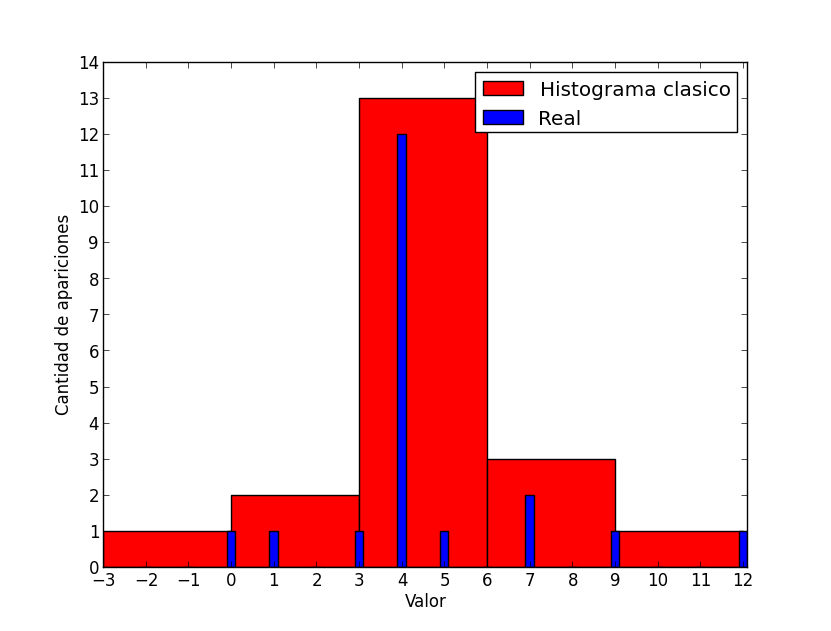
\includegraphics[width=0.6\textwidth]{./imagenes/ejb1_ejemplo_classic_y_real.png}
  \caption{Comparacion Classic vs. Real}
\end{figure}


Tomemos como ejemplo la \textit{selectividad de 5}.
En la \textit{figura 1} vemos que la selectividad es de $0.65$ pues queda agrupado junto
con \textit{4} que es un valor que aparece muchas veces. Sin embargo, los datos reales nos
indican que deberia ser \textit{0.05} ya que tiene pocas apariciones.

Como vemos este es un caso \textbf{no favorable} para \textbf{Classic Histogram} y
muestra la ventaja de controlar la altura de los \textit{bins}.


\begin{figure}[h!]
  \centering
  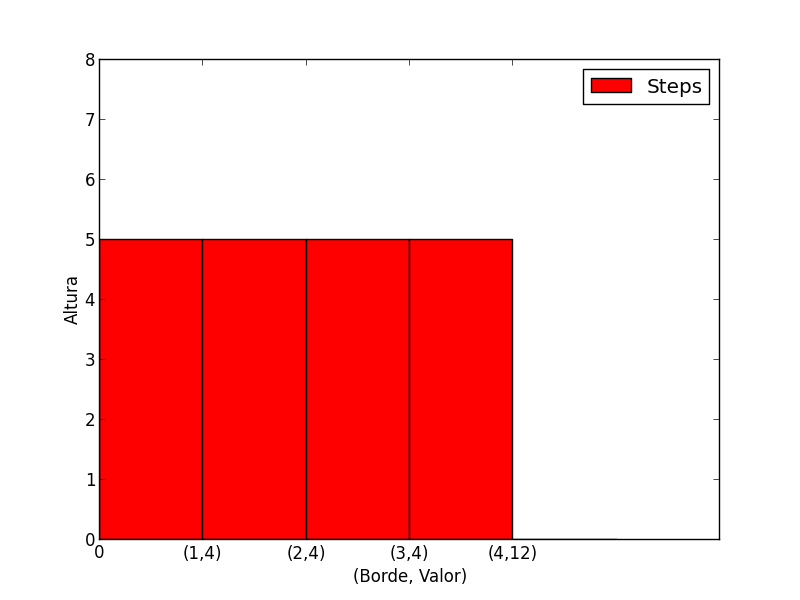
\includegraphics[width=0.6\textwidth]{./imagenes/ejb1_ejemplo_steps.png}
  \caption{Distribution Steps}
\end{figure}


Para el mismo ejemplo, examinamos la \textit{selectividad de 5} nuevamente con el nuevo histograma.
Podemos observar que esta vez, la selectividad es de $0.25$. Si bien tambien se desvia del
valor real ($0.05$), la diferencia del error es significativa comparada con \textbf{Classic Histogram}.


Basándose en el ejemplo planteado, se observa que el comportamiento de los distintos estimadores
depende de la distribición de los datos.
Por ejemplo, cuando los datos están agrupados, \textbf{Distribucion Steps} brinda un menor
error en la estimación pero, cuando los datos estan dispersos el error del estimador es
mucho mayor que el que presenta \textbf{Classic Histogram}.

A continuación se experimentará con datos que siguen una distribución uniforme o normal.


[Ale dice q aclaremos q esto se explica mas adelante]


\subsubsection{Generación casos de prueba}
Los casos de prueba que se van a utilizar para el análisis del comportamiento de ambos
estimadores se generarán de manera aleatoria. Se define una función que genera números
aleatorios que siguen una distribucion normal o uniforme.



\subsubsection{Factores}

Debido a la estructura que se utiliza para construir los estimadores y el algoritmo de
construcción de los mismos, se podrá afirmar que:

\paragraph{Classic Histogram}
% Usamos un diccionario
\begin{itemize}

\item Costo de creación de estimador:
\begin{equation}
O(b * n + n )
\end{equation}
\begin{equation}
O(b * n)
\end{equation}

Siendo \textit{n} la cantidad total de tuplas existentes en la base de datos.
Por el otro lado, \textit{b} representa el valor pasado en \textbf{PARAM}.
Como se recorre toda la tabla por cada dato que se requiere para la tabla del estimador,
se deberá considerar un costo de $b * n$. Por otro lado, también se requiere almacenar en
la estructura del estimador, el máximo, mínimo y la cantidad total de tuplas, lo cual es
una búsqueda que realiza el motor de bases de datos en tiempo lineal.

\item Costo espacial del estimador:
\begin{equation}
O(2 * b + 3 ) \\
\end{equation}
\begin{equation}
O(2 * b)
\end{equation}
Se utiliza un diccionario que presenta un costo espacial del valor pasado en PARAM por dos,
ya que por cada bin se almacen dos valores más (la cantidad y el acumulado hasta ese valor).
Por otro lado, se requere almacenar el máximo, mínimo y la cantidad total.

\item Costo de consulta:
\begin{equation}
O(1)
\end{equation}
Lo único se se requere es el acceso al diccionario, lo cual presenta un costo constante.

\end{itemize}
\paragraph{Distribution Steps}
% Usamos un Array

\begin{itemize}

\item Costo de creación del estimador:
\begin{equation}
O(n*log(n) + n + n)
\end{equation}
\begin{equation}
O(n*log(n))
\end{equation}
El algoritmo consiste en el ordenamiento de las tuplas de acuerdo a la columna pasada por
parámetro. El ordanamiento lo realiza el motor de la base de datos en costo $O(n*log(n))$.
Por otro lado se deberá calcular el máximo, mínimo y total de tuplas existentes en la base.

\item Costo espacial del estimador:
\begin{equation}
O(b + 1) \\
\end{equation}
\begin{equation}
O(b)
\end{equation}
Se requiere unicamente almacenar un array con las tuplas que se encuentran en las distintas
posiciones de los steps. Además, se deberá almacenar la cantidad de tuplas totales
existentes en la tabla pasada por parámetro.

\item Costo de consulta:
\begin{equation}
O(n)
\end{equation}
Tanto para una búsqueda por igualdad o por menor, se deberá recorrer el array buscando
el valor de tupla deseado.

\end{itemize}

\subsection{Ejercicio b2 - Cambiar nombre}

\subsubsection{Classic Histogram}

Como explicamos anteriormente, el \textbf{param} indica la cantidad de bins que generamos.

Suponemos que cuando \textbf{param} toma un valor mas grande, disminuye el error en la estimación,
pues agrupa menor cantidad de valores por \textit{bin}.

Ademas, suponemos que la distribucion de los datos no influencia en el resultado. Si bien
el histograma puede tener menor error con una determinada distribucion, la cantidad de
\textit{bins} suponemos que produciria una reduccion de error mas significativa.

Veamos el siguiente gráfico que muestra el error promedio que comete el histograma variando
la cantidad de \textit{bins}.

\begin{figure}[h!]
  \centering
  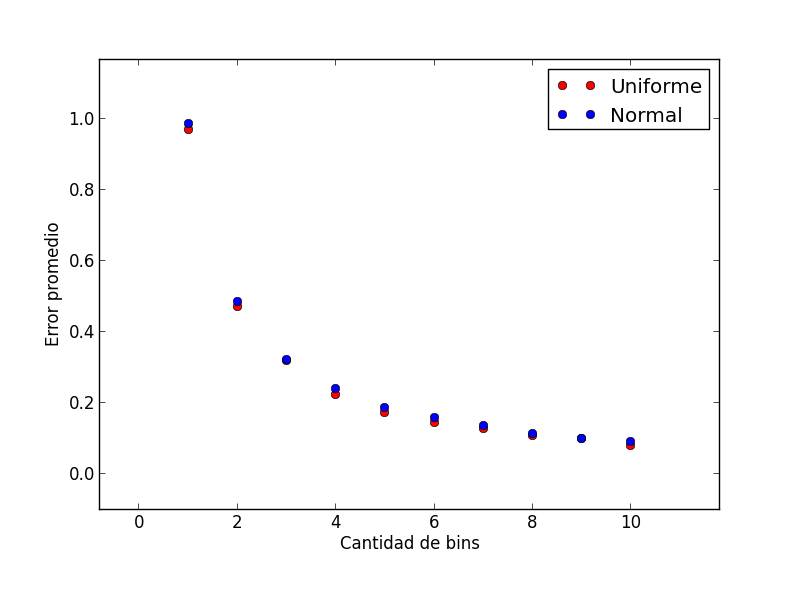
\includegraphics[width=0.6\textwidth]{./imagenes/ejb2_classic_parameter_variation.png}
  \caption{Classic Histogram - Variacion del parametro}
\end{figure}


Como era de esperar, mejora a medida que agrandamos el \textbf{param}.
Esto es porque separa mejor los casos y entonces se tiene una estimacion mas precisa.
Sin embargo, por cada incremento de \textit{bin}, el costo se incrementa pues se requiere
mas espacio para almacenar las estadisticas.

Si hacemos que $param \rightarrow n$ (siendo n la cantidad de valores distintos), nos
daria la estimación perfecta, pero con un costo altisimo tanto espacial como computacional.



\subsubsection{Distribution Steps}

Para este histograma, partimos con una suposicion similar, pues la diferencia es que mientras
mas \textit{steps} se crean, mas chicos son los \textit{bins} que agrupan valores.


Veamos el siguiente gráfico que muestra el error promedio que comete el histograma variando
la cantidad de \textit{bins}.

\begin{figure}[h!]
  \centering
  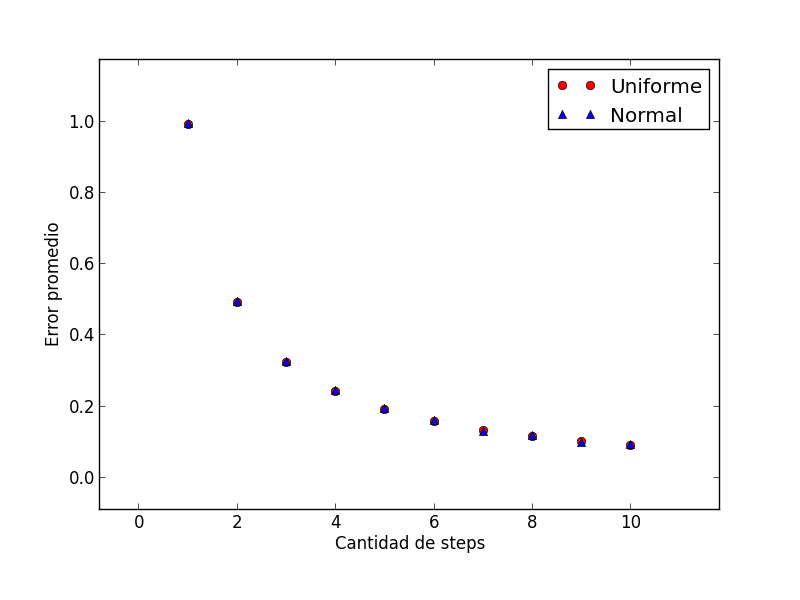
\includegraphics[width=0.6\textwidth]{./imagenes/ejb2_step_parameter_variation.png}
  \caption{Distribution Steps - Variacion del parametro}
\end{figure}

Nuevamente nuestra hipotesis se confirma. El costo tambien se ve incrementado por
la cantidad de \textit{steps}.




\subsubsection{Group}

A diferencia de los histogramas anteriores, este cuenta con dos parametros.

\begin{itemize}
  \item size - cantidad de bins
  \item threshold - maximo error permitido
\end{itemize}

Como este Histograma es una modificacion de \textit{Classic Histogram}, obtendriamos la misma
conclusion al variar el \textbf{size}, el equivalente de \textbf{params}.

Por lo tanto, nos queda ver como evoluciona la estimacion cuando modificamos el
\textbf{threshold}, es decir aumentando y disminuyendo el maximo error permitido.

Esperamos ver, que a medida que se achica el \textbf{threshold}, la selectividad es mas precisa.


Veamos el siguiente gráfico que muestra el \textit{maximo error} que comete el histograma
variando el \textbf{threshold}.

\begin{figure}[h!]
  \centering
  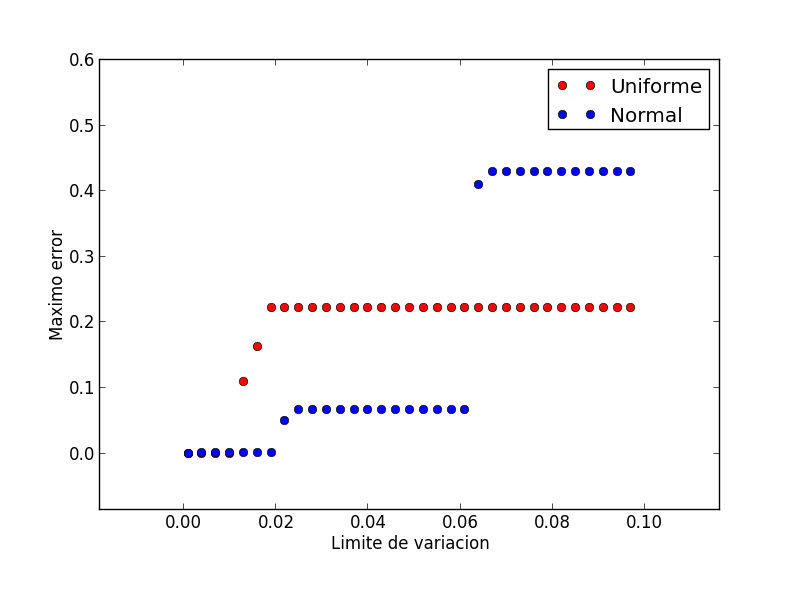
\includegraphics[width=0.6\textwidth]{./imagenes/ejb2_group_parameter_variation.png}
  \caption{Distribution Group - Variacion del threshold}
\end{figure}


En el caso de la distribucion uniforme, para sorpresa nuestra, el maximo error llega a un
techo y no sigue creciendo. No lo supusimos desde el principio, pero cobra sentido si
recordamos que los datos provienen de una distribucion uniforme, donde la varianza no es
grande. Por eso solo podemos apreciar las grandes mejoras, con un \textbf{threshold} muy pequeño.

Para la distribucion normal, el grafico si muestra como mejora la presicion o como se pierde
para los distintos valores del \textbf{threshold}. Recordemos que una vez cruzado el
\textbf{threshold} definimos un \textit{bin} por cada valor distinto, esto nos da mayor
precision pero aumenta la memoria consumida por la estructura y al mismo tiempo el tiempo
consumido para generarla.



\subsection{Ejercicio 1 b 3}

--- Analice cómo impacta el uso de distintas distribuciones como entrada para los tres estimadores. ---


Para el estimador GROUP es muy importante conocer la varianza de la distribucion pues, nos
basamos en ella para encontrar un valor aceptable para el error.

Es decir, nuestro estimador ofrece una mejora al Classic Histogram cuando la distribucion
de los datos tiene un valor elevado de Varianza.






/////// NO CAMBIA



\subsubsection{Distribución Uniforme}

Partimos con una base de datos cuya información cumple con una distribución uniforme.

\begin{figure}[h!]
  \centering
  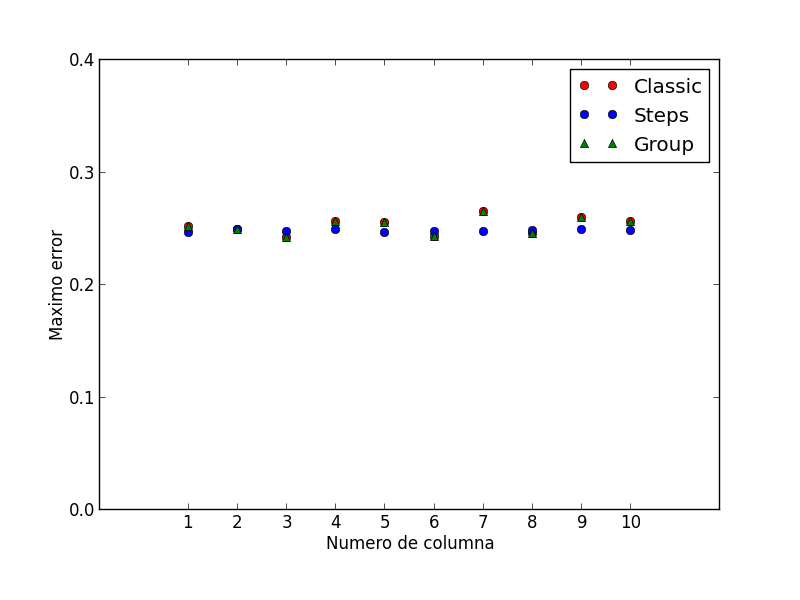
\includegraphics[width=0.6\textwidth]{./imagenes/ejb3_uniforme.png}
  \caption{Comparacion Classic vs. Step para distribucion uniforme}
\end{figure}


Con respecto al error de factor en la estimacion, ambos estimadores no difieren
significativamente en sus resultados. Dado que al tener los datos distribuidos de forma
uniforme, la probabilidad de cada tupla es $1/n$, siendo $n$ la cantidad total de tuplas de la tabla.

( Para rango |a-b|/(max - min))


Debido a que se los compara con igual cantidad de steps, entonces la altura, en el caso de
\textbf{Classic Histogram}, y el ancho, en el \textbf{Distribution Steps}, son similares.
En el caso de \textbf{Group Histogram}, al ser una especializacion del Classic, tambien tiene
una altura similar.

Sin embargo, teniendo en cuenta el factor de costos de creación, el estimador
\textbf{Distribution Steps} es más costoso. El motivo principal es debido al ordenamiento
de los datos antes de construir el histograma requerido. Luego sigue el \textbf{Group Histogram}
pues requiere \textit{bins} particulares para los algunos elementos. Y por ultimo se encuentra el \textit{Classic Histogram}.

En conclusión, para datos que cumplen una distribución uniforme, sugerimos implementar
\textbf{Classic Histogram}, debido al menor costo de construcción del histograma.


\subsubsection{Distribución Normal}

Partimos con una base de datos que la información sigue una distribución normal.

Se hicieron experimentos modificando la varianza para observar cual es el comportamiento de los tres estimadores.

Se realizaron diversos graficos comparandolos en simultaneo teniendo en cuenta el parametro dicho.
A continuacion se presenta un ejemplo con una varianza igual a $0,05$. 

\begin{figure}[h!]
  \centering
  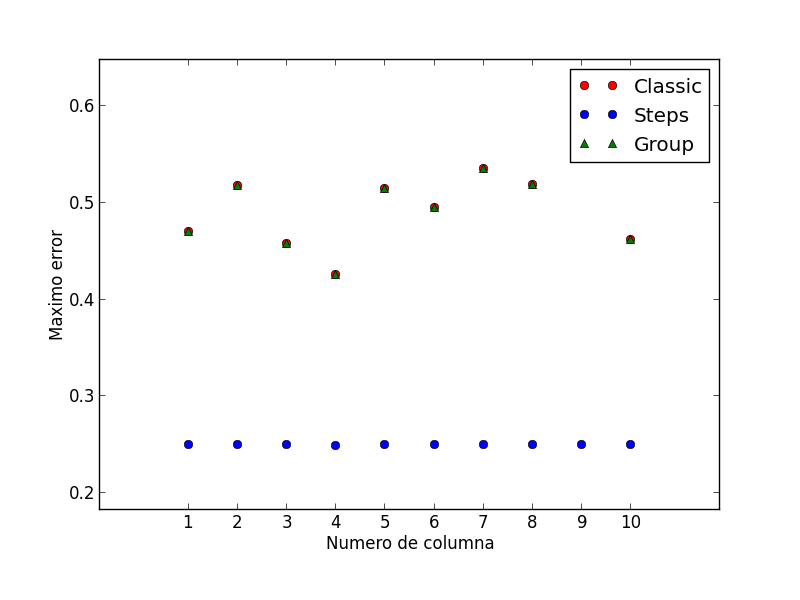
\includegraphics[width=0.6\textwidth]{./imagenes/ejb2_normal_t_005.png}
  \caption{Comparacion Classic vs. Step para distribucion normal}
\end{figure}

Como se puede ver, con una varianza chica, el error maximo es muy bajo en el estimador de distribution steps. En cambio, para classic histograms y group histrograms es mas alto, aunque similar entre si. Esto se debe a que los resultados de gruop histograms son muy similares con respecto a classic histograms si no se acepta un error alto, ya que no se agregan bins. De esta manera no se puede notar la mejora del estimador.


Luego se presenta un experimento realizado con una varianza igual a $0,03$. 

\begin{figure}
  \centering
  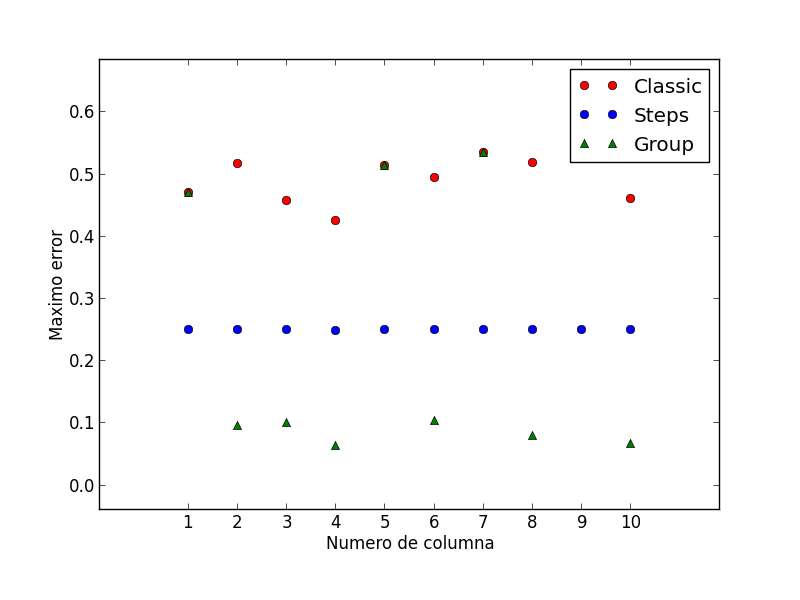
\includegraphics[width=0.6\textwidth]{./imagenes/ejb2_normal_t_003.png}
  \caption{Comparacion Classic vs. Step para distribucion normal}
\end{figure}

Con respecto al grafico anterior se puede observar una diferencia del maximo error para algunas columnas en el estimador Group Histograms. En los otros dos estimadores el error maximo sigue siendo similar ya que el cambio en la varianza no modifica sus resultados. 

La diferencia en group histograms se debe a que al disminuir la varianza se le esta indicando al algoritmo que el error maximo debe ser menor. Por lo tanto el estimador generara un mayor numero de bins aumentando asi la precision en los calculos. No ocurre una mejora para todas las columnas, ya que la varianza no es lo suficientemente baja. 


A continucacion, se muestra otro grafico con una varianza de $0.01$

\begin{figure}
  \centering
  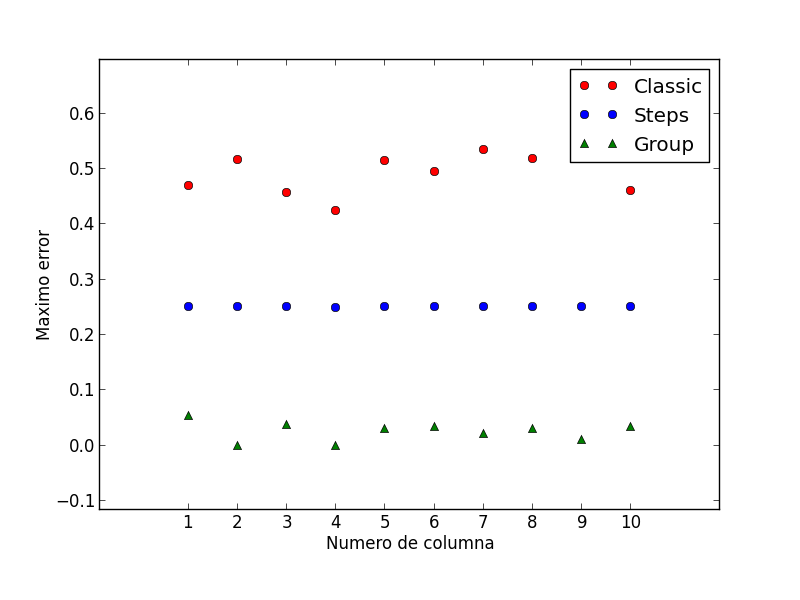
\includegraphics[width=0.6\textwidth]{./imagenes/ejb2_normal_t_001.png}
  \caption{Comparacion Classic vs. Step para distribucion normal}
\end{figure}

La diferencia con el grafico anterior es notoria con respecto a group histograms. Esto se debe a que la varianza pasa por parametro es lo suficientemente baja para que se genere una mejora en todas las columnas de la base de datos. 

\end{document}
